\textbf{See the instruction for questions \inteval{\value{question}+1} to \inteval{\value{question}+3}.}

A circuit consists of a resistor $R$, an inductor $L$, and an open switch $S$ connected in series with a battery. The switch is then closed at time $t=0$.

% Multiple Choice Question 29
\begin{questions}\setcounter{question}{28}\question
If the current in the circuit is $I$ at time $t$, what energy is stored in the circuit in addition to that stored in the battery?

\begin{oneparchoices}
\choice $L I$
\choice $I^{2} R$
\choice $\dfrac{1}{2} L I^{2}$
\choice $L I+I^{2} R$
\choice $\dfrac{1}{2} L I^{2}+I^{2} R$
\end{oneparchoices}\end{questions}

\begin{figure}[H]
    \center
    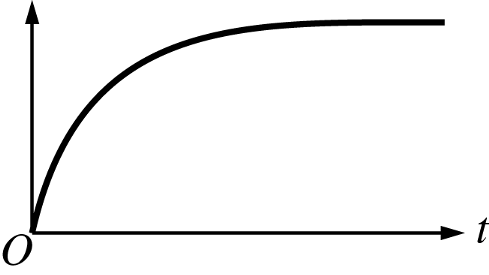
\includegraphics[scale=0.25]{images/img-011-021.png}
\end{figure}

% Multiple Choice Question 30
\begin{questions}\setcounter{question}{29}\question
Which of the following quantities could be represented as a function of time by the graph shown above?
\begin{enumerate}
    \item The potential difference across the resistor
    \item The potential difference across the inductor
    \item The current in the circuit
\end{enumerate}

\begin{oneparchoices}
\choice I only
\choice II only
\choice I and III only
\choice II and III only
\choice I, II, and III
\end{oneparchoices}\end{questions}

% Multiple Choice Question 31
\begin{questions}\setcounter{question}{30}\question
The change in current when the switch is closed is determined by the inductive time constant $\tau$. If the inductance is doubled and the resistance is halved, the new inductive time constant $\tau^{\prime}$ equals

\begin{oneparchoices}
\choice $\dfrac{1}{4} \tau$
\choice $\dfrac{1}{2} \tau$
\choice $\tau$
\choice $2 \tau$
\choice $4 \tau$
\end{oneparchoices}\end{questions}

